\documentclass[11pt]{article}
\usepackage[croatian]{babel}
\usepackage[utf8]{inputenc}
\usepackage{amsmath}
\usepackage{amsfonts}
\usepackage{amssymb}
\usepackage{graphicx}
\usepackage{xfrac}
\usepackage{enumerate}
\usepackage[T1]{fontenc}
\newcommand{\HRule}{\rule{\linewidth}{0.5mm}}
%%% END Article customizations

%%% The "real" document content comes below...


%\date{} % Activate to display a given date or no date (if empty),
         % otherwise the current date is printed 
\begin{document}
\begin{titlepage}
\begin{center}

\LARGE Sveučilište u Zagrebu \\[0.5cm] Prirodoslovno -- matematički fakultet \\[0.5cm] Matematički odsjek\\[2cm]

\Large Statistički praktikum 1\\[0.5cm]

% Title
\HRule \\[0.4cm]
{ \huge \bfseries Seminar - 36. zadatak}\\[0.4cm]

\HRule \\[6.5cm]

% Autor i mentor -> postavljanje ovoga na dno stranice...
\begin{minipage}{0.4\textwidth}
\begin{flushleft} \large
\emph{Student:\\}
Hermina Petric Maretić\\
\emph{e-mail:\\}
hpetricmaretic@gmail.com\\
\end{flushleft}
\end{minipage}
\begin{minipage}{0.4\textwidth}
\begin{flushright} \large
\emph{Mentori:\\}
Prof.dr.sc. Miljenko Huzak\\
Dipl.ing. Snježana Lubura\\
\end{flushright}
\end{minipage}


\vfill
% Bottom of the page
{\large Zagreb, \today}

\end{center}
\end{titlepage}
\section*{Tekst zadatka}

List indijanske penjačice Pharabitis nil može biti šaren ili jednoličan, te istovremeno blijed ili
normalne boje. Postavljeno je pitanje jesu li te dvije karakteristike nezavisne. Prijašnji
eksperimenti su pokazali da ce prilikom križanja dviju biljaka određenog tipa lišća mladica s
vjerojatnosti $\sfrac{1}{4}$ biti blijeda (a normalne boje s vjerojatnosti $\sfrac{3}{4}$ ). Isto tako lišće mladica ce s
vjerojatnosti $\sfrac{1}{4}$ biti šareno (a s vjerojatnosti $\sfrac{3}{4}$ jednolično). Na slučajan način prikupljen je
uzorak od 290 mladica indijske penjačice. Rezultati opažanja dviju spomenutih karakteristika
nalaze se u tablici (N.T.J. Bailey Mathematical Theory of Genetic Linkage, Clarendon Press,
Oxfrord).
\begin{center}
\begin{tabular}{|c|c|c|}
\hline 
 & normalne boje & blijedo \\ 
\hline 
jednolično & 187 & 35 \\ 
\hline 
šareno & 37 & 31 \\ 
\hline 
\end{tabular} \\
\end{center}
\begin{enumerate}[(a)]

\item Neka je X stanje prve karakteristike (šareno ili lišće jednolične boje), a Y stanje druge
karakteristike (blijedo lišće ili normalne boje). Na osnovi danog uzorka, procijenite zajedničku
razdiobu varijabli X i Y, tj. procijenite razdiobu vektora (X,Y) i grafički je predstavite.
Također, graficki je usporedite s razdiobom u kojoj su X i Y nezavisne, a marginalne razdiobe
su u skladu s prijašnjim saznanjima.
\item Testirajte da li su X i Y nezavisne s pretpostavljenim marginalnim razdiobama kao u
tekstu zadatka.
\item Odredite jakost testa iz (b) uz značajnost 5\%
\item Prema jednoj drugoj teoriji, razdioba od (X,Y) je oblika
\begin{center}
\begin{tabular}{|c|c|c|}
\hline 
X \ Y & normalne boje & blijedo \\ 
\hline 
jednolično & $\sfrac{9}{16} + \theta $ & $\sfrac{3}{16} - \theta $ \\ 
\hline 
šareno & $\sfrac{3}{16} - \theta $ & $\sfrac{1}{16} + \theta $ \\ 
\hline 
\end{tabular} 
\end{center}
gdje je H nepoznati parametar. Odredite parametarski prostor i pomoću 
$ \chi ^2$-testa testirajte
tu hipotezu, pri čemu nepoznati parametar procjenite minimum $ \chi ^2$-metodom.
\item Procijenite nepoznati prametar iz modela u (d) metodom maksimalne vjerodostojnosti
i usporedite ga s minimum $ \chi ^2$-procjenom

\end{enumerate}

\section*{Rješenje}
\begin{enumerate}[(a)]
\item Na osnovu danog uzroka želimo procijeniti razdiobu vektora (X,Y). Da bismo dobili procijenjenu razdiobu, podijelit ćemo opažene frekvencije s veličinom uzorka.
\begin{verbatim}
podaci=matrix(c(187,37,35,31),2,2)
> n=sum(podaci)
> f=c(podaci)
> pkapa=podaci/n
> pkapa
          [,1]      [,2]
[1,] 0.6448276 0.1206897
[2,] 0.1275862 0.1068966

\end{verbatim}
Procijenjenu razdiobu možemo i grafički prikazati:
\begin{verbatim}
pkapa=c(pkapa)
png('1.png')
barplot(c(pkapa),names.arg=c("JN","ŠN","JB","ŠB"),ylim=c(0,0.7),
col="darkgreen",main="Procijenjena razdioba vektora (X,Y)")
dev.off()
\end{verbatim}
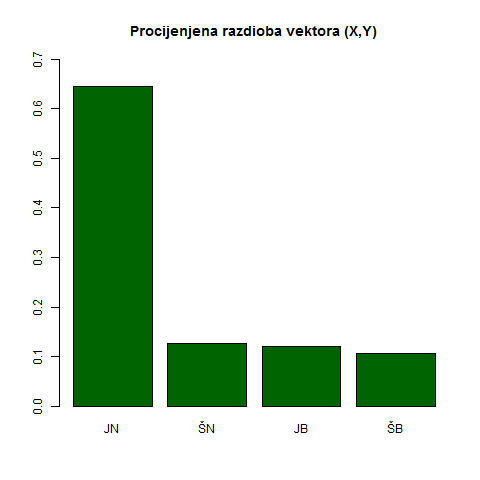
\includegraphics[scale=0.45]{1.png}\\\\
Iz teksta zadatka vidimo da su dosadašnja mjerenja pokazala sljedeće marginalne distribucije:
\begin{verbatim}
> x1=c(3/4,1/4)
> y1=c(3/4,1/4)
> x1
[1] 0.75 0.25
> y1
[1] 0.75 0.25
\end{verbatim}
U slučaju nezavisnosti slučajnih varijabli, distribucija cijelog slučajnog vektora određena je marginalnim distribucijama, jer tada vrijedi jednakost $f_{X,Y}(x,y)=f_{X}(x)*f_{Y}(y)$.
\begin{verbatim}
> nez1=x1%*%t(y1)
> nez1
       [,1]   [,2]
[1,] 0.5625 0.1875
[2,] 0.1875 0.0625
\end{verbatim} 
Sada možemo grafički usporediti te dvije razdiobe.
\begin{verbatim}
> lista=matrix(numeric(0),2,4)
> lista[1,]=pkapa
> lista[2,]=c(nez1)
> png('2.png')
> barplot(lista,beside=TRUE,names.arg=c("JN","ŠN","JB","ŠB"),
ylim=c(0,0.7),col=c("cornsilk", "lavender"),
main="Usporedba procijenjene i nezavisne razdiobe",
legend.text=list("Slucajni uzorak","Nezavisna razdioba"))
> dev.off()
\end{verbatim}
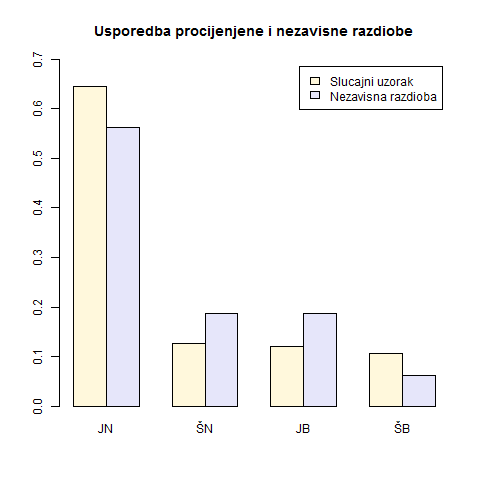
\includegraphics[scale=0.45]{2.png}\\
\item Postavljamo hipoteze:\\
$ H_{0} $= X i Y su nezavisne s pretpostavljenim marginalnim razdiobama\\
$ H_{0} $= X i Y nisu neazavisne s pretpostavljenim marginalnim razdiobama\\
Za testiranje koristimo Pearsonov $\chi^2$-test o pripadnosti distribuciji s testnom statistikom 
$H=\sum_{i=1}^{r} \sum_{j=1}^{c} \dfrac{(f_{i,j}-f_{i,j}')^2}{f_{i,j}'} \sim \chi^2(r*c-d-1)$, gdje je d = broj procijenjenih parametara = 0.\\
Računamo kritično područje i p-vrijednost:
\begin{verbatim}
> fnez=nez1*n
> fnez
        [,1]   [,2]
[1,] 163.125 54.375
[2,]  54.375 18.125
> fnez=c(fnez)
> h=sum(((f-fnez)^2)/fnez)
> h
[1] 25.09579
> c=qchisq(0.95,3) 
> c
[1] 7.814728
> pv=1-pchisq(h,3)
> pv
[1] 1.474459e-05
\end{verbatim}

Kritično područje je $[7.815,\infty\rangle$, a vrijednost testne statistike h=25.096. Jasno je da testna statistika upada u kritično područje, pa odbacujemo nultu hipotezu, odnosno na razini značajnosti od 5\% zaključujemo da X i Y nisu nezavisne. P vrijednost od $1.47*10^{-5}$ nam govori da bismo nultu hipotezu odbacili na svim razinama značajnosti većim od tog broja, odnosno gotovo uvijek.\\

\item Želimo odrediti jakost testa iz (b) uz razinu značajnosti $\alpha$=5\%. Postavljamo hipoteze:\\
$H_{0}: p=p^{(0)}$\\
$H_{1}: p=p^{(0)} - \frac{1}{\sqrt{n}} \delta$, za neki $\delta\neq 0$\\
Testna statistika je $H=\sum_{i=1}^{r} \sum_{j=1}^{c} \dfrac{(f_{i,j}-f_{i,j}')^2}{f_{i,j}'} \sim \chi^2(r*c-d-1)$\\
Ako vrijedi hipoteza $H_{1}$, tada je $H\sim A_{\chi^2} (k-1,\lambda)$, gdje je $\lambda=\sum_{k=1}^k \dfrac{\delta_{i}^2}{p_{i}^0}$ parametar
necentralnosti.\\
Tada funkciju jakosti Pearsonovog $\chi^2$-testa možemo prikazati ovako:\\
$\gamma(\lambda)=P(H\geq \chi^2(k-1)|p=p^0-\frac{1}{\sqrt{n}}*\delta)=1-P_{\chi^2(k-1,\lambda)}(\chi_{\alpha}^2 (k-1))$\\
Iz definicije koeficijnta necentralnosti $\lambda$ jasno je da je $lambda \geq 0$. Definiramo funkciju jakosti testa u R-u i prikazujemo njezin graf:\\
\begin{verbatim}
> hi=qchisq(0.95,3)
> hi
[1] 7.814728
> gama=function(lambda){
+ return(1-pchisq(hi,3,lambda))
+ }
> png('3.png')
> plot(gama,type="l",xlim=c(0,100),main="Graf funkcije jakosti 
testa",xlab="Parametar necentralnosti lambda",ylab="gama(lambda)")
> dev.off()
\end{verbatim}
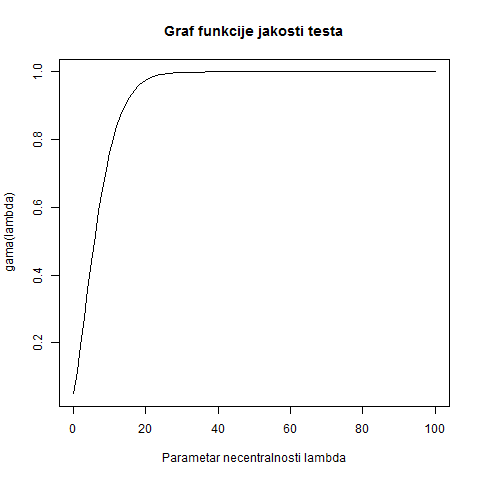
\includegraphics[scale=0.45]{3.png}\\
Tražimo minimum i točku u kojoj se on postiže:
\begin{verbatim}
> optim(0,gama,method=c("L-BFGS-B"),lower=0,upper=0.05)
$par
[1] 0

$value
[1] 0.05

$counts
function gradient 
       1        1 

$convergence
[1] 0

$message
[1] "CONVERGENCE: NORM OF PROJECTED GRADIENT <= PGTOL"
\end{verbatim}
Vidimo da se minimum postiže u točki 0 i da iznosi 0.05. To proizlazi iz činjenice da hipoteza $H_{0}$ govori upravo da je $\lambda=0$ i iz činjenice da test ima razinu značajnosti 5\%.\\
\item Poznato je da sve vrijednosti u distribuciji moraju biti između 0 i 1. Da bi predloženi model to zadovoljavao, moramo uvesti ograničenja na parametar $\theta$:\\
$\sfrac{9}{16} + \theta \in [0,1]$\\
$\sfrac{3}{16} - \theta \in [0,1]$\\
$\sfrac{1}{16} + \theta \in [0,1]$\\
Ovim smo uvjetima zapravo konstruirali sustav nejednadžbi. Njegovim rješavanjem dobivamo $\theta \in [\sfrac{-1}{16}, \sfrac{3}{16}]$\\
Taj interval nazivamo parametarskim prostorom.\\
Procijenimo sada parametar $\theta$ minimum $\chi^2$-metodom. Metoda se temelji na tome da za funkciju $h(\theta):\Theta\rightarrow R$, $h(\theta)=\sum_{i=1}^{k} \sum_{j=1}^{c} \dfrac{(f_{i,j}-f_{i,j}'(\theta))^2}{f_{i,j}'(\theta)}$ tražimo vrijednost $\hat{\theta}$ u kojoj ona postiže minimum.\\
Definiramo funkciju h:
\begin{verbatim}
> h=function(theta){
+ p2=c(9/16+theta,3/16-theta,3/16-theta,1/16+theta)
+ n2=p2*290
+ return(sum(((f-n2)^2)/n2))
+ }
\end{verbatim}
Prikazujemo je grafički u ovisnosti o parametru $\theta$ i tražimo minimum:
\begin{verbatim}
> png('4.png')
> plot(Vectorize(h),type="l",xlim=c(-1/16,3/16),
main="Graf funkcije h(theta)")
> dev.off()
> optim(0.05,h,method="L-BFGS-B",lower=0,upper=0.15)
$par
[1] 0.05861457

$value
[1] 0.9015172

$counts
function gradient 
       9        9 

$convergence
[1] 0

$message
[1] "CONVERGENCE: REL_REDUCTION_OF_F <= FACTR*EPSMCH"

> theta1=optim(0.05,h,method="L-BFGS-B",lower=0,upper=0.15)$par
> theta1
[1] 0.05861457
\end{verbatim}
Kao što i otprilike vidimo na grafu, minimum se postiže u točki 0.0586, pa je baš to naš $\hat{\theta}$. \\
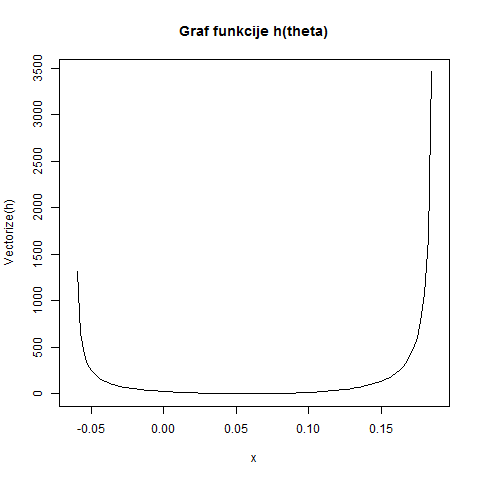
\includegraphics[scale=0.45]{4.png}\\
Sada testiramo hipotezu da je razdioba našeg slučajnog vektora iz zadanog modela. Iskoristimo procijenjeni parametar $\theta$ i provodimo $\chi^2$-test s k-d-1=r*c-1-1=2 (d=1 jer imamo jedan procijenjeni parametar) stupnja slobode. 
\begin{verbatim}
> f2=matrix(c(9/16+theta1,3/16-theta1,3/16-theta1,1/16+theta1),2,2)
> f2

          [,1]      [,2]
[1,] 0.6211146 0.1288854
[2,] 0.1288854 0.1211146
> hop=h(theta1)
> hop
[1] 0.9015172
> pv=1-pchisq(hop,2)
> pv
[1] 0.6371446
\end{verbatim}
P-vrijednost je velika, pa ne možemo odbaciti hipotezu o pripadnosti zadanom modelu.\\

\item Želimo procijeniti nepoznati parametar $\theta$ iz (d) metodom maksimalne
vjerodostojnosti. Definiramo funkciju vjerodostojnosti $L:\Theta \rightarrow R$, sa $L(\theta)=\prod_{i=1}^{n} f(x_{i}|\theta)$. Tražimo $\theta$ koji maksimizira ovu funkciju i zovemo ga procjenom metodom maksimalne vjerodostojnosti.\\
Definiramo funkciju L(u kodu mle) i prikazujemo njen graf:
\begin{verbatim}
> mle=function(theta){
+ return ((9/16 + theta)^187 * (3/16 - theta)^35 *
(3/16 - theta)^37 * (1/16+ theta)^31)
+ }
> plot(mle,type="l",xlim=c(-1/16,3/16),
main="Graf funkcije vjerodostojnosti")
\end{verbatim}
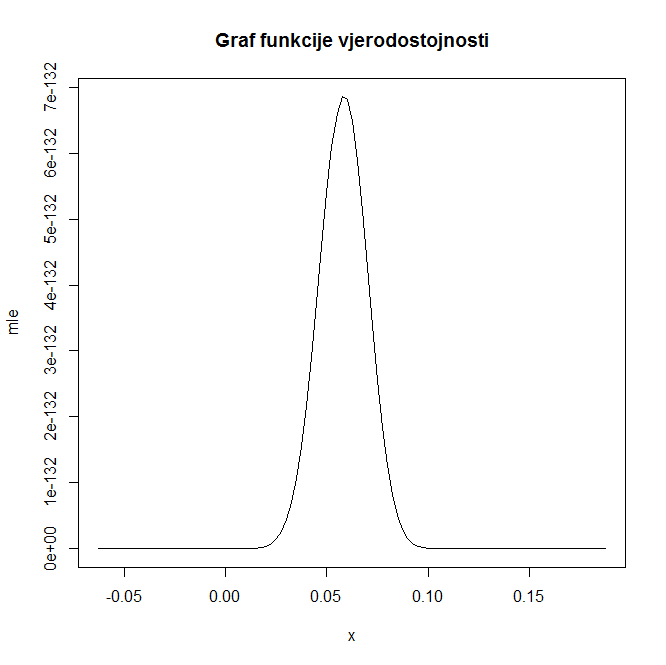
\includegraphics[scale=0.4]{45.png}\\
Kako bismo našli maksimum, deriviramo funkciju i prikazujemo graf derivacije.
\begin{verbatim}
> D(expression((9/16 + theta)^187 * (3/16 - theta)^35 *
(3/16 - theta)^37 * (1/16+ theta)^31),"theta")
((187 * (9/16 + theta)^186 * (3/16 - theta)^35 - (9/16 + theta)^187 * 
    (35 * (3/16 - theta)^34)) * (3/16 - theta)^37 - (9/16 + theta)^187 * 
    (3/16 - theta)^35 * (37 * (3/16 - theta)^36)) * (1/16 + theta)^31 + 
    (9/16 + theta)^187 * (3/16 - theta)^35 * (3/16 - theta)^37 * 
        (31 * (1/16 + theta)^30)
> der=function(theta){
+ ((187 * (9/16 + theta)^186 * (3/16 - theta)^35 - (9/16 + theta)^187 * 
+ (35 * (3/16 - theta)^34)) * (3/16 - theta)^37 - (9/16 + theta)^187 * 
+ (3/16 - theta)^35 * (37 * (3/16 - theta)^36)) * (1/16 + theta)^31 + 
+ (9/16 + theta)^187 * (3/16 - theta)^35 * (3/16 - theta)^37 * 
+ (31 * (1/16 + theta)^30)
+ }
> plot(der,type="l",xlim=c(-1/16,3/16),
main="Graf derivacije funkcije vjerodostojnosti")
\end{verbatim}
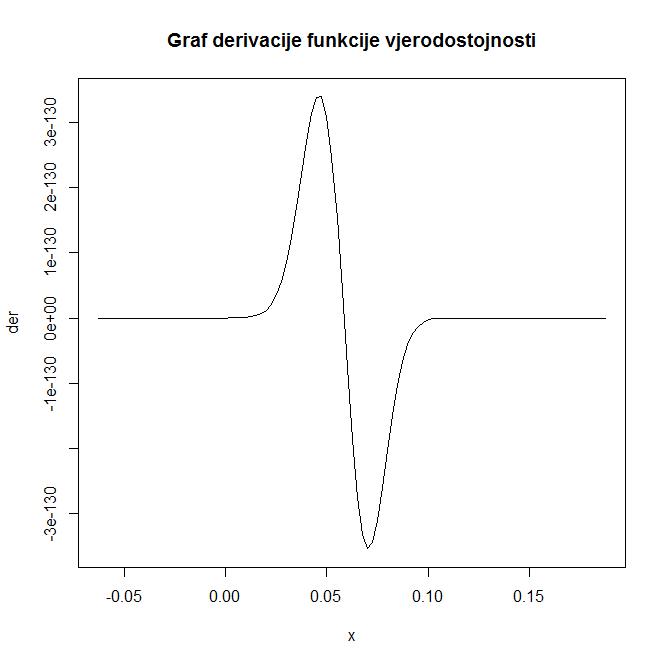
\includegraphics[scale=0.4]{5.png}\\
Sada otprilike znamo gdje je nultočka, pa tražimo nultočku na tom području. Time smo pronašli $\hat{\theta}$. Sad dobivene podatke uvrštavamo u model i i uspoređujemo distribucije dobivene procjenom nepoznatog parametra metodom maksimalne vjerodostojnosti i minimum $\chi^2$-procjenom.
\begin{verbatim}
> theta2=uniroot(der,c(0,0.1))$root
> theta2
[1] 0.05840407
> f3=matrix(c(9/16+theta2,3/16-theta2,3/16-theta2,
1/16+theta2),2,2)
> f3
          [,1]      [,2]
[1,] 0.6209041 0.1290959
[2,] 0.1290959 0.1209041
> usporedba=matrix(numeric(8),2,4)
> usporedba[1,]=c(f2)
> usporedba[2,]=c(f3)
> usporedba
          [,1]      [,2]      [,3]      [,4]
[1,] 0.6211146 0.1288854 0.1288854 0.1211146
[2,] 0.6209041 0.1290959 0.1290959 0.1209041
> barplot(usporedba,beside=TRUE,names.arg=c("JN","ŠN","JB","ŠB"),
ylim=c(0,0.7),col=c("cornsilk", "lavender"),
main="Usporedba razdioba slucajnog vektora (X,Y)",
legend.text=list("Minimum hi-kvadrat metoda",
"Metoda maksimalne vjerodostojnosti"))
\end{verbatim}
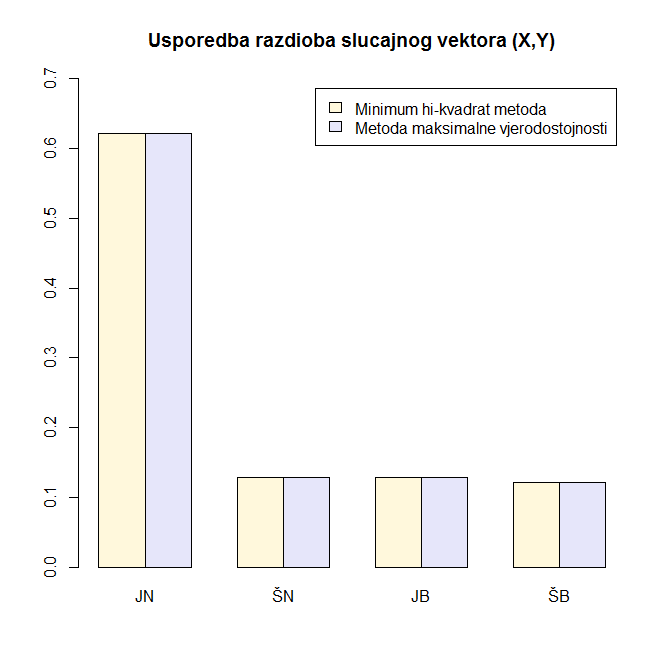
\includegraphics[scale=0.4]{6.png}\\
Kao što smo vidjeli i iz ispisa dviju različitih procjena parametra $\theta$, procjene su vrlo slične.
\end{enumerate}
\end{document}